\documentclass[11pt,a4paper]{article}

\usepackage[T1]{fontenc}
\usepackage[utf8]{inputenc}
\usepackage{lmodern}
\usepackage[margin=2.5cm]{geometry}
\usepackage{amsmath,amssymb}
\usepackage{graphicx}
\usepackage{float}
\usepackage{needspace}
\usepackage{booktabs}
\usepackage{tabularx}
\usepackage{enumitem}
\usepackage{xcolor}
\usepackage{listings}
\usepackage[font=small,labelfont=bf]{caption}
\usepackage{tikz}
\usetikzlibrary{arrows.meta,positioning,calc}
\usepackage{pgfplots}
\pgfplotsset{compat=1.16}
\usepackage[hidelinks]{hyperref}

\graphicspath{{figures/}}
\newcolumntype{Y}{>{\raggedright\arraybackslash}X}
\setlist{itemsep=2pt,topsep=4pt}
\setlength{\parindent}{0pt}
\setlength{\parskip}{6pt}

\lstset{
  basicstyle=\ttfamily\footnotesize,
  keywordstyle=\bfseries,
  commentstyle=\itshape,
  stringstyle=\ttfamily,
  columns=fullflexible,
  keepspaces=true,
  breaklines=true,
  frame=lines,
  framesep=4pt,
  showstringspaces=false,
  xleftmargin=2pt,
  xrightmargin=2pt
}

\begin{document}

% ------------------------------------------------------------ title page
\begin{titlepage}
\centering
\vspace*{3cm}
{\Large FCV Lab 11: Mini Project (Phase II)\par}
\vspace{1.5cm}
{\LARGE\bfseries Vision-Assisted Survivor Localisation in Maritime Search and Rescue using Texture-Anomaly Modelling\par}
\vspace{2cm}
{\large Final Report\par}
\vspace{2cm}
{\large\textbf{Team Members}\par}
\vspace{0.5cm}
\begin{tabular}{ll}
\toprule
Name & Registration no. \\
\midrule
Tanish Hemant Kuvar & 240962540 \\
M. Vishal Kumar & 240962546 \\
Samyak Jain & 240962638 \\
\bottomrule
\end{tabular}
\vspace{1cm}

{\large Section AIML-A\par}
\vfill
{\large November 2026\par}
\end{titlepage}

% ------------------------------------------------------------ abstract
\section*{Abstract}
\addcontentsline{toc}{section}{Abstract}

This project finds people in the water from aerial RGB imagery and reached 92.4\% recall@5 on a synthetic benchmark, using only classical computer vision and no training data. People in the water often cover fewer than 16 pixels, too few for appearance-based recognition. The system therefore models the water rather than the person.

Each frame passes through six stages: illumination normalisation, Gabor and uniform LBP texture description, chi-square anomaly scoring, glint suppression, morphological shape filtering and temporal tracking. The output is a ranked shortlist of at most $k$ regions per frame, drawn as an overlay in a Tkinter operator GUI.

On 6 synthetic sequences (60 frames each, 739 annotated people), the full system scored 51.7\% precision and 1.77 false alarms per frame at $k = 5$. Recall rose to 99.3\% once the tracker had warmed up. Throughput was about 2.7 frames/s at $1280 \times 720$ on a laptop CPU. These numbers validate the pipeline end to end; they do not measure real-world performance, which still has to be tested on public datasets.

\clearpage
\tableofcontents
\clearpage

% ------------------------------------------------------------ problem
\section{Problem Statement}

The task is to give a rescue operator a short, ranked list of places to look in each aerial frame, so that a person in the water is not lost among waves, glitter and foam. Three things make this hard:

\begin{itemize}
  \item \textbf{Small targets.} 618 of the 739 annotated people in the benchmark measure under 16 px (square root of box area).
  \item \textbf{Moving clutter.} Waves, sun glint, whitecaps and debris all differ from calm water, and all change from frame to frame.
  \item \textbf{No fixed appearance.} A partly submerged person can show only a head, and clothing colour varies.
\end{itemize}

\subsection{Objectives}

\begin{enumerate}
  \item Return at most $k$ candidate regions per frame, each with a confidence value.
  \item Work without training data, using classical operations only.
  \item Expose every intermediate stage and parameter, so an operator can inspect and tune the system.
  \item Measure performance with recall@$k$, false alarms per frame, precision and stage-by-stage ablation.
\end{enumerate}

\subsection{System Requirements}

\begin{table}[H]
\centering
\small
\caption{Functional, non-functional, software and input requirements.}
\label{tab:requirements}
\begin{tabularx}{\textwidth}{@{}lYY@{}}
\toprule
Type & Requirement & How the project meets it \\
\midrule
Functional & Accept video, an image folder or a single image & \texttt{run} command and GUI file loaders \\
Functional & Output a ranked top-$k$ shortlist as an overlay and a CSV & \texttt{run -{}-output -{}-csv}; GUI shortlist table \\
Functional & Let the operator inspect stages and tune parameters & GUI stage selector, 16 sliders, config save and load \\
Functional & Evaluate against annotated data & \texttt{evaluate} command; COCO JSON and YOLO txt loaders \\
Non-functional & Run on a CPU with no GPU & About 2.7 frames/s at $1280 \times 720$ on a laptop CPU \\
Non-functional & Be repeatable and tested & 40 passing unit and integration tests \\
Software & Python with NumPy $\geq$ 1.24, OpenCV $\geq$ 4.8, Pillow $\geq$ 9.0, Matplotlib $\geq$ 3.7, pytest $\geq$ 7.0; Tkinter for the GUI & \texttt{requirements.txt} \\
Input & Daylight aerial RGB imagery of open water & Night and thermal imagery are out of scope \\
\bottomrule
\end{tabularx}
\end{table}

% ------------------------------------------------------------ methodology
\section{Methodology}

The method describes normal sea texture from the frame itself and flags what deviates, so it needs no labelled training images. Stages 1 to 5 run on each frame, and stage 6 uses the history across frames. Figure~\ref{fig:pipeline} shows the data flow.

\begin{figure}[H]
\centering
\resizebox{\textwidth}{!}{%
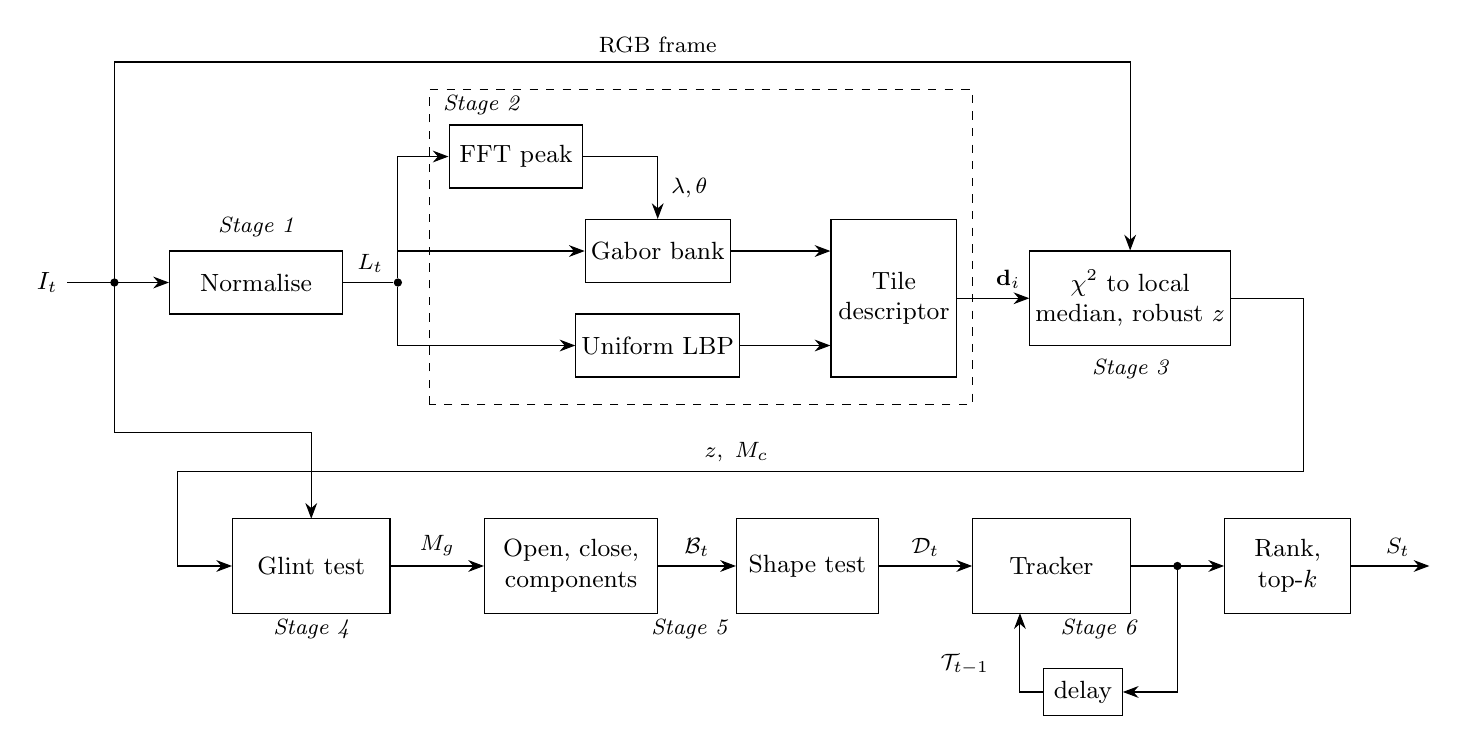
\begin{tikzpicture}[
  >={Stealth[length=2mm]},
  line width=0.4pt,
  every node/.style={font=\small},
  blk/.style={draw,rectangle,minimum height=8mm,align=center,inner sep=2pt},
  sig/.style={font=\footnotesize},
  stg/.style={font=\footnotesize\itshape},
  dot/.style={circle,fill,inner sep=0pt,minimum size=3pt}
]
% row 1
\node[blk,minimum width=22mm] (norm) at (1.9,0) {Normalise};
\node[dot] (split) at (3.7,0) {};
\node[blk,minimum width=17mm] (fft) at (5.2,1.6) {FFT peak};
\node[blk,minimum width=18mm] (gabor) at (7,0.4) {Gabor bank};
\node[blk,minimum width=18mm] (lbp) at (7,-0.8) {Uniform LBP};
\node[blk,minimum width=16mm,minimum height=20mm] (tile) at (10,-0.2) {Tile\\descriptor};
\node[blk,minimum width=22mm,minimum height=12mm] (chi) at (13,-0.2) {$\chi^2$ to local\\median, robust $z$};

% stage 2 frame
\draw[dashed] (4.1,-1.55) rectangle (11.0,2.45);
\node[stg,anchor=west] at (4.15,2.25) {Stage 2};
\node[stg] at (1.9,0.7) {Stage 1};
\node[stg] at (13,-1.1) {Stage 3};

% input and feeds
\node[anchor=east] (inp) at (-0.5,0) {$I_t$};
\draw[->] (-0.5,0) -- (norm.west);
\node[dot] at (0.1,0) {};
\draw[->] (0.1,0) -- (0.1,2.8) -- (13,2.8) -- (chi.north);
\node[sig,above] at (7,2.8) {RGB frame};
\draw[->] (0.1,0) -- (0.1,-1.9) -- (2.6,-1.9) -- (2.6,-3.0);

% stage 1 to stage 2
\draw (norm.east) -- (split);
\node[sig,above] at (3.35,0) {$L_t$};
\draw[->] (split) |- (fft.west);
\draw[->] (split) |- (gabor.west);
\draw[->] (split) |- (lbp.west);
\draw[->] (fft.east) -| (gabor.north);
\node[sig,anchor=west] at (7.05,1.2) {$\lambda,\theta$};
\draw[->] (gabor.east) -- (gabor.east -| tile.west);
\draw[->] (lbp.east) -- (lbp.east -| tile.west);
\draw[->] (tile.east) -- (chi.west);
\node[sig,above] at (11.45,-0.2) {$\mathbf{d}_i$};

% wrap to row 2
\node[blk,minimum width=20mm,minimum height=12mm] (glint) at (2.6,-3.6) {Glint test};
\node[blk,minimum width=22mm,minimum height=12mm] (morph) at (5.9,-3.6) {Open, close,\\components};
\node[blk,minimum width=18mm,minimum height=12mm] (shape) at (8.9,-3.6) {Shape test};
\node[blk,minimum width=20mm,minimum height=12mm] (track) at (12,-3.6) {Tracker};
\node[blk,minimum width=16mm,minimum height=12mm] (rank) at (15,-3.6) {Rank,\\top-$k$};
\node[blk,minimum width=10mm,minimum height=6mm] (delay) at (12.4,-5.2) {delay};

\draw[->] (chi.east) -- (15.2,-0.2) -- (15.2,-2.4) -- (0.9,-2.4) -- (0.9,-3.6) -- (glint.west);
\node[sig,above] at (8,-2.4) {$z,\ M_c$};

\draw[->] (glint.east) -- (morph.west);
\node[sig,above] at (4.2,-3.6) {$M_g$};
\draw[->] (morph.east) -- (shape.west);
\node[sig,above] at (7.5,-3.6) {$\mathcal{B}_t$};
\draw[->] (shape.east) -- (track.west);
\node[sig,above] at (10.4,-3.6) {$\mathcal{D}_t$};
\draw[->] (track.east) -- (rank.west);
\node[dot] at (13.6,-3.6) {};
\draw[->] (13.6,-3.6) -- (13.6,-5.2) -- (delay.east);
\draw[->] (delay.west) -- (11.6,-5.2) -- (11.6,-4.2);
\node[sig,below] at (10.9,-4.6) {$\mathcal{T}_{t-1}$};
\draw[->] (rank.east) -- (16.8,-3.6);
\node[sig,above] at (16.4,-3.6) {$S_t$};

\node[stg] at (2.6,-4.4) {Stage 4};
\node[stg] at (7.4,-4.4) {Stage 5};
\node[stg] at (12.6,-4.4) {Stage 6};
\end{tikzpicture}%
}
\caption{Block diagram of the pipeline. $I_t$: input frame; $L_t$: normalised lightness; $\lambda,\theta$: dominant wavelength and orientation; $\mathbf{d}_i$: descriptor of tile $i$; $z$: anomaly map; $M_c$, $M_g$: candidate mask before and after the glint test; $\mathcal{B}_t$: blobs; $\mathcal{D}_t$: detections; $\mathcal{T}_{t-1}$: tracks from the previous frame; $S_t$: shortlist. Optional camera-motion compensation is not drawn.}
\label{fig:pipeline}
\end{figure}

The filtering operations in stages 1, 2, 4 and 5 are detailed in Section~\ref{sec:enhancement}. This section covers how they are combined into a decision.

\subsection{Anomaly Scoring (Stage 3)}

Each overlapping tile has a descriptor made of mean Gabor energies and a 59-bin uniform LBP histogram~\cite{ojala}. The reference for normal sea is the median descriptor over $9 \times 9$-tile windows. A median stays clean when a person or a boat covers some tiles, and the local window adapts to near and far field.

Each tile is compared with its reference using the chi-square distance, computed separately for LBP and for reference-normalised Gabor energy:
\begin{equation}
\chi^2(a, b) = \frac{1}{2} \sum_i \frac{(a_i - b_i)^2}{a_i + b_i}
\end{equation}

The two distances are put on one scale with a robust z-score and averaged with equal weight:
\begin{equation}
z = \frac{d - \mathrm{median}(d)}{1.4826 \cdot \mathrm{MAD}(d)}
\end{equation}

Each pixel takes the maximum $z$ of the tiles covering it, and the anomalous region is $z > 3$. Inside it, candidate pixels are those whose Lab colour differs from the median-filtered local sea colour by more than $\mathrm{median} + 4\sigma_{\mathrm{MAD}}$.

\subsection{Temporal Association and Ranking (Stage 6)}

Detections are linked between frames by greedy nearest neighbour around a constant-velocity prediction, within a 40 px radius. A track is promoted after 5 hits if its drift is coherent, meaning $\exp(-\mathrm{spread} / 6\,\mathrm{px}) \geq 0.25$, where spread is the RMS deviation of step velocities from their mean. Gaps of up to 3 frames are tolerated, which covers a head briefly under a wave.

Shown tracks are ranked by this confidence, then multiplied by 0.8 per missed frame:
\begin{equation}
\mathrm{conf} = 0.4 \cdot \mathrm{conf}_{\mathrm{anomaly}} + 0.6 \cdot \frac{\min(\mathrm{hits}, 10)}{10} \cdot \mathrm{coherence}
\end{equation}

\subsection{Evaluation Protocol}

The benchmark has 6 rendered sequences of 60 frames at $1280 \times 720$ and 10 fps, with 739 annotated people. It covers altitudes of 50--150 m, calm to rough sea, strong sun glitter, a dark-clothed person and a panning camera.

A prediction counts as a hit when its centre lies within $\max(8\,\mathrm{px}, \max(w, h))$ of the ground-truth centre, because IoU is very harsh on boxes of 10--30 px. Steady-state figures leave out the first 4 frames of each sequence, when the tracker cannot yet have promoted anything.

\subsection{Results}

The full system found 92.4\% of people in a five-item shortlist with 1.77 false alarms per frame. \textbf{All results below are from the synthetic benchmark.} They show that the pipeline and evaluation work end to end, and they are not a claim about real-world performance.

\begin{figure}[H]
\centering
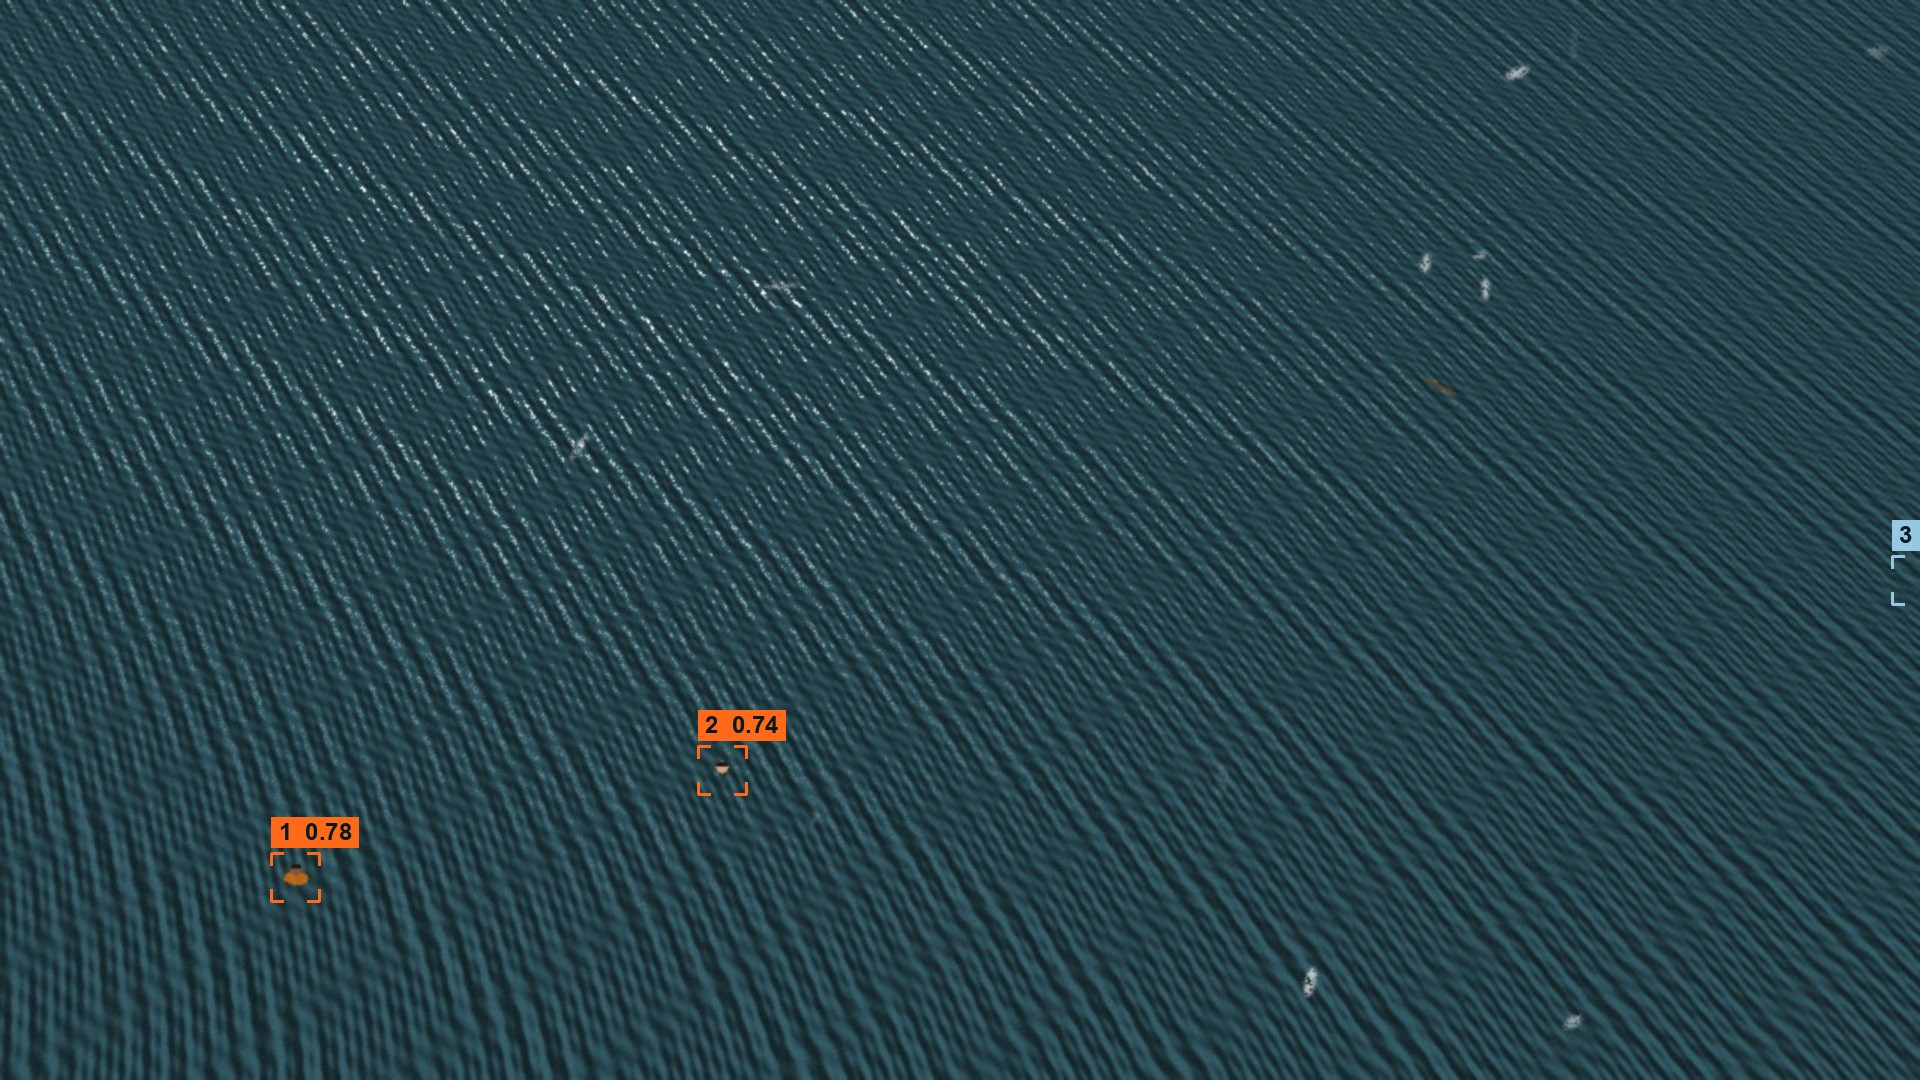
\includegraphics[width=0.72\textwidth]{result_seq05.jpg}
\caption{Output on sequence 5, frame 31. Orange brackets mark hits, and ranks and confidences are shown beside them.}
\label{fig:result}
\end{figure}

\begin{table}[H]
\centering
\small
\caption{Ablation at $k = 5$. FA: false alarms; SS: steady state.}
\label{tab:ablation}
\begin{tabularx}{\textwidth}{@{}Yrrrrrr@{}}
\toprule
Run & Recall@5 & Precision@5 & FA/frame & SS recall@5 & SS FA/frame & Frames/s \\
\midrule
\textbf{Full system} & \textbf{92.4\%} & \textbf{51.7\%} & \textbf{1.77} & \textbf{99.3\%} & \textbf{1.90} & \textbf{2.67} \\
Without temporal stage & 89.2\% & 40.2\% & 2.73 & 88.7\% & 2.80 & 2.64 \\
Without glint suppression & 92.4\% & 51.2\% & 1.81 & 99.3\% & 1.94 & 2.75 \\
Without morphology and shape filter & 92.4\% & 45.7\% & 2.50 & 99.3\% & 2.68 & 2.65 \\
\bottomrule
\end{tabularx}
\end{table}

Switching off one stage at a time shows what each contributes:

\begin{itemize}
  \item \textbf{Temporal stage:} false alarms per frame fall 35\%, from 2.73 to 1.77, and precision rises from 40.2\% to 51.7\%.
  \item \textbf{Morphology and shape filter:} false alarms per frame fall from 2.50 to 1.77.
  \item \textbf{Glint suppression:} only a small change here, from 1.81 to 1.77. The synthetic glitter specks are 1--3 px, so opening and the minimum-area limit remove most of them first.
\end{itemize}

\begin{figure}[H]
\centering
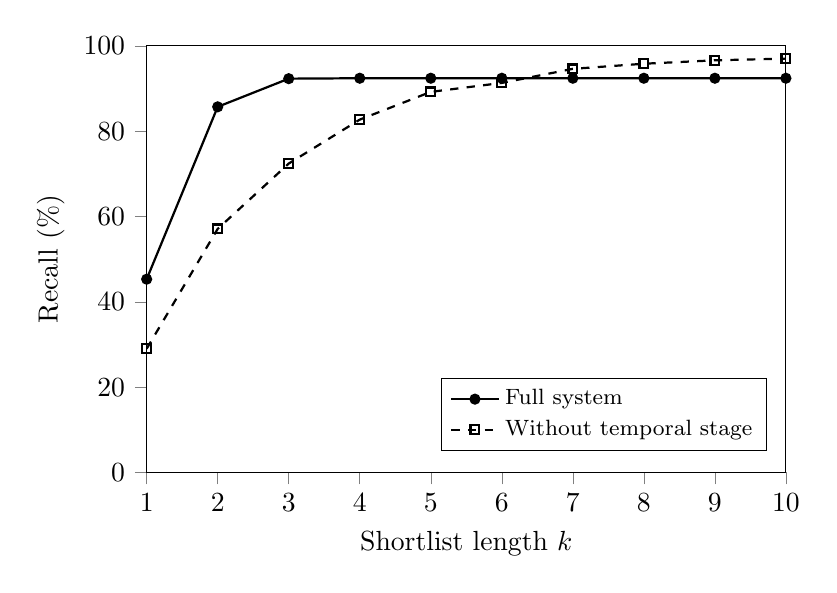
\begin{tikzpicture}
\begin{axis}[
  width=0.8\textwidth,
  height=7cm,
  xlabel={Shortlist length $k$},
  ylabel={Recall (\%)},
  xmin=1, xmax=10,
  ymin=0, ymax=100,
  xtick={1,2,3,4,5,6,7,8,9,10},
  ytick={0,20,40,60,80,100},
  tick align=outside,
  tick pos=left,
  grid=none,
  legend style={at={(0.97,0.05)},anchor=south east,font=\footnotesize,draw=black},
  legend cell align=left,
  every axis plot/.append style={line width=0.8pt,black},
]
\addplot[mark=*,mark size=1.6pt] coordinates {
  (1,45.3) (2,85.7) (3,92.3) (4,92.4) (5,92.4) (6,92.4) (7,92.4) (8,92.4) (9,92.4) (10,92.4)
};
\addlegendentry{Full system}
\addplot[dashed,mark=square,mark options={solid},mark size=1.6pt] coordinates {
  (1,29.0) (2,57.1) (3,72.4) (4,82.7) (5,89.2) (6,91.3) (7,94.6) (8,95.8) (9,96.6) (10,97.0)
};
\addlegendentry{Without temporal stage}
\end{axis}
\end{tikzpicture}
\caption{Recall against shortlist length on the synthetic benchmark (360 frames, 739 annotated people).}
\label{fig:recall}
\end{figure}

Persistence lifts people above short-lived clutter in the ranking, so recall@3 rises from 72.4\% to 92.3\% (Figure~\ref{fig:recall}). The cost is the warm-up: nothing can be shown in a sequence's first 4 frames, so the full system stays at 92.4\% and the run without tracking overtakes it at $k \geq 7$. At $k = 5$ the steady-state recall of the full system is 99.3\%. Most frames hold 2--3 people, so recall@1 cannot exceed about 45\%.

\begin{figure}[H]
\centering
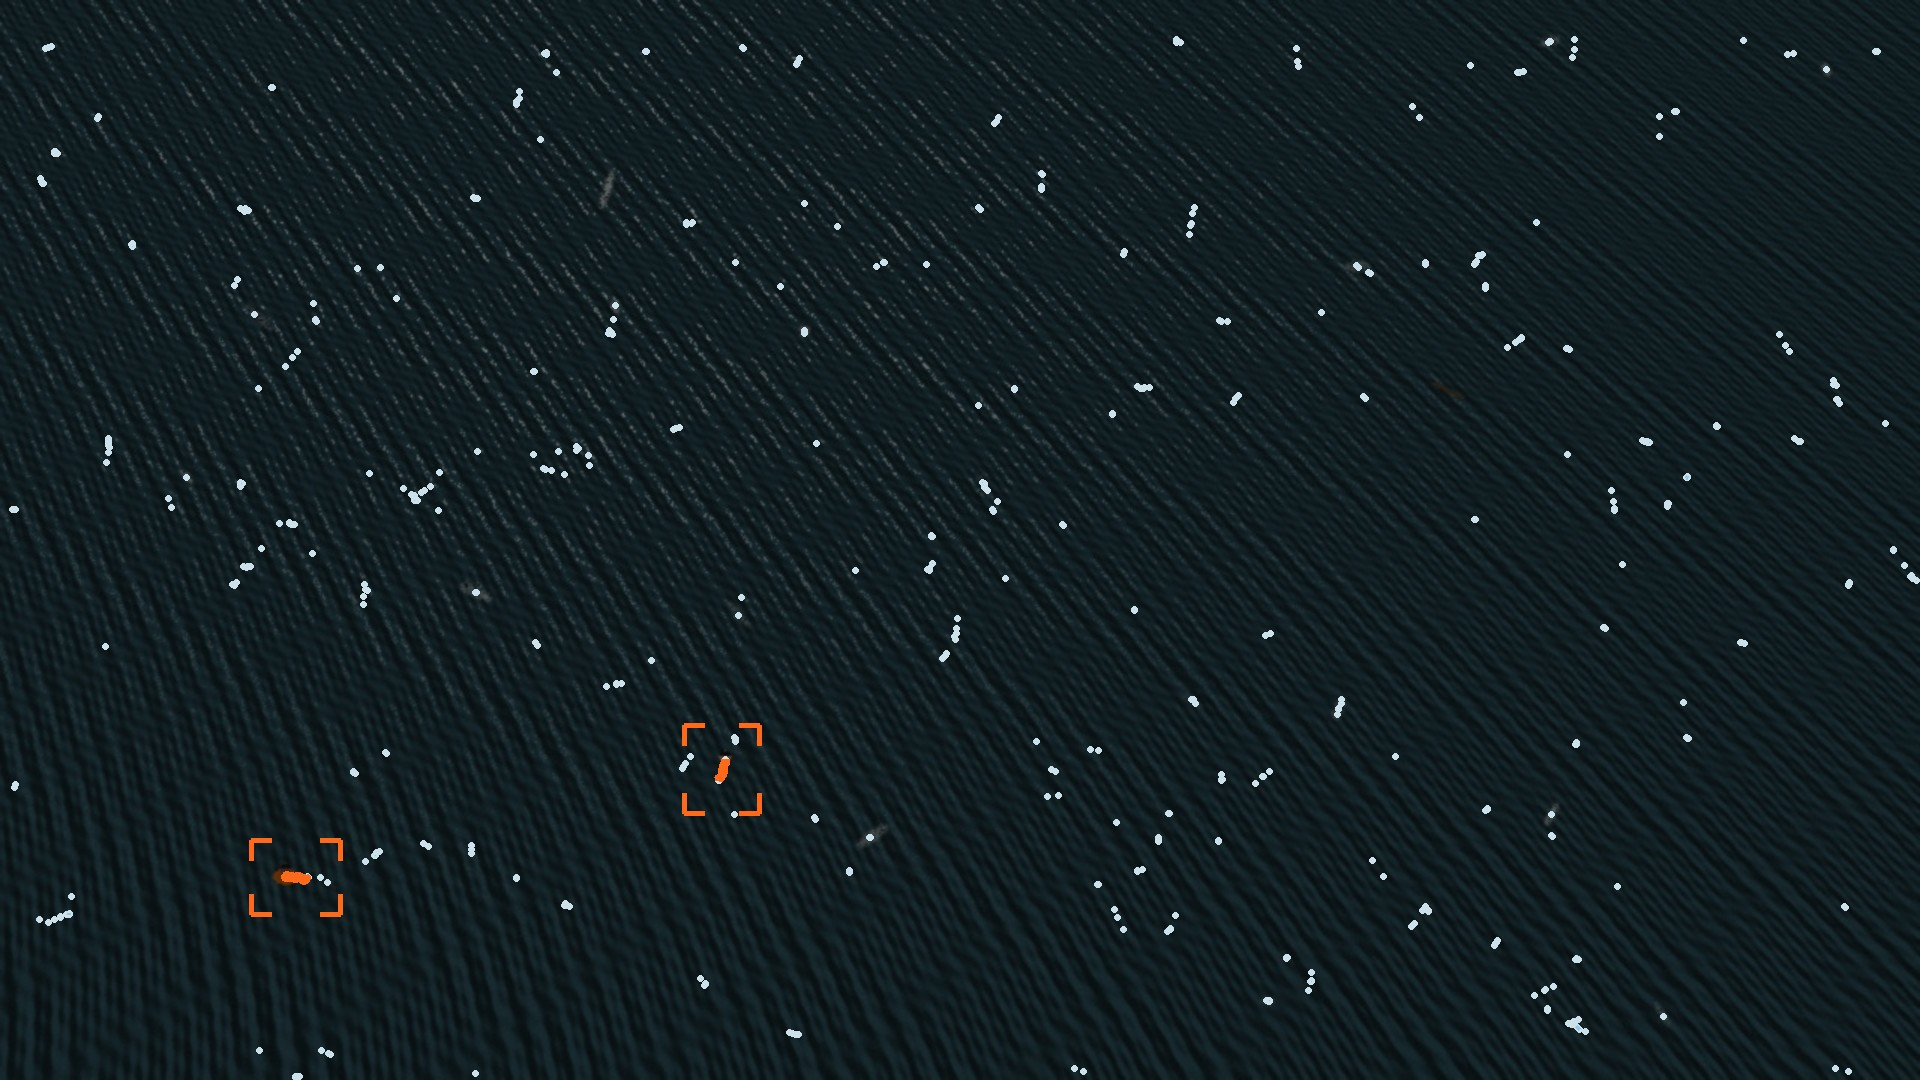
\includegraphics[width=0.72\textwidth]{tracks_final.jpg}
\caption{All detections across 60 frames of sequence 5. The two people form continuous tracks (orange); everything else appears briefly (pale dots).}
\label{fig:tracks}
\end{figure}

Figure~\ref{fig:tracks} shows why tracking works. The sequence produced 665 raw detections, yet each person's track stayed on the shortlist for 56 frames, and no other track lasted more than 7.

Recall@5 stayed steady across conditions, at 93.2\% below 60 m, 92.9\% at 60--100 m, 89.0\% at 100--140 m and 93.3\% at 140 m and above. It was 92.2\% for targets under 16 px ($n = 618$) and 93.4\% for 16--32 px ($n = 121$).

We inspected all 11 false alarms at frame 31 across the six sequences by eye: 3 looked like debris, 3 like whitecaps and 5 showed nothing visible. Debris is a real anomaly but not a person. One of the few steady-state misses is sequence 3, frames 27--30, where a person has a whitecap right beside them; that the whitecap is the cause has not been confirmed.

\subsection{Limitations}

\begin{itemize}
  \item \textbf{Synthetic data only.} Real-world performance still has to be measured. Loaders are ready for SeaDronesSee~\cite{seadronessee} and MOBDrone~\cite{mobdrone} (COCO JSON) and AFO~\cite{afo} (YOLO txt).
  \item \textbf{Dark, colourless targets} give weak colour and texture contrast.
  \item \textbf{Very bright white or grey clothing} can be removed by the glint test.
  \item \textbf{Non-sea content} such as a coastline or large ship can contaminate the local reference.
  \item \textbf{Persistent clutter}, such as long-lived whitecaps or debris, can be promoted to a track.
  \item \textbf{Warm-up:} nothing is shown in the first 4 frames of a sequence.
  \item \textbf{Camera motion:} phase correlation handles translation only, not rotation or zoom.
  \item \textbf{Hand-tuned parameters} may need retuning for a new camera or sea state.
  \item \textbf{Night and thermal imagery} are out of scope, because the colour test assumes daylight RGB.
\end{itemize}

% ------------------------------------------------------------ UI
\section{UI Design}

The operator GUI, built with Tkinter, puts the frame in the centre, the controls on the left and the ranked answer on the right. An operator reads the shortlist first, and a developer can open any stage to see why a box did or did not appear.

\begin{figure}[H]
\centering
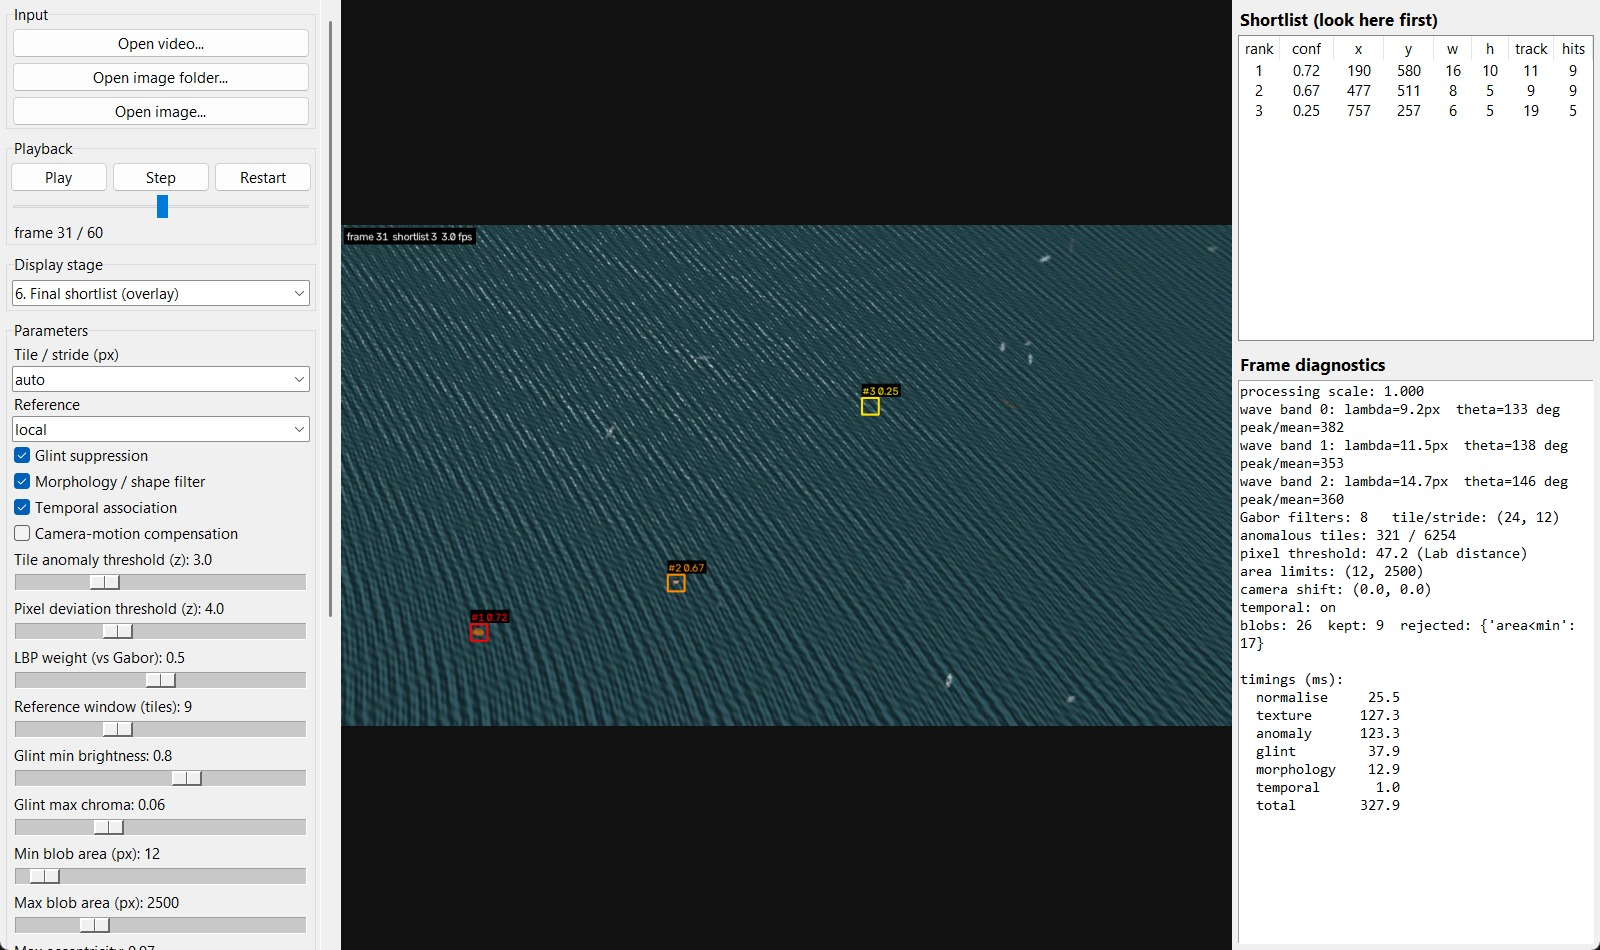
\includegraphics[width=\textwidth]{gui.jpg}
\caption{Main window on the final overlay, sequence 5, frame 31. The shortlist table gives rank, confidence, box, track id and hits.}
\label{fig:gui}
\end{figure}

\begin{figure}[H]
\centering
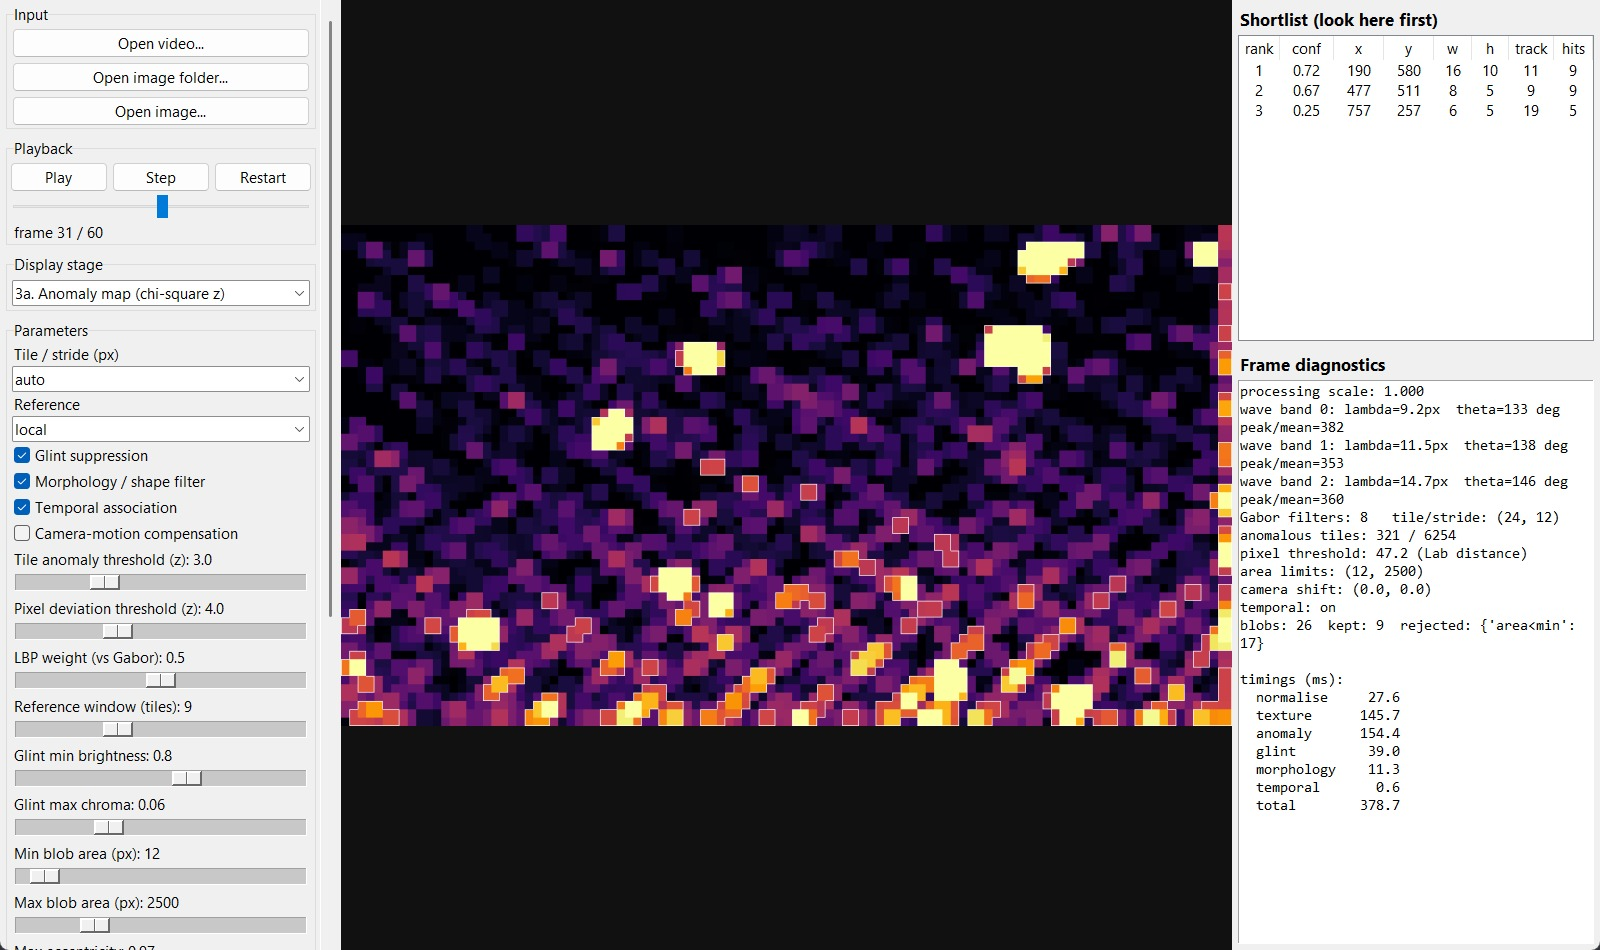
\includegraphics[width=\textwidth]{gui_anomaly.jpg}
\caption{The same frame with the display stage set to 3a, the anomaly map. Parameters and diagnostics stay in place.}
\label{fig:guianomaly}
\end{figure}

\begin{table}[H]
\centering
\small
\caption{GUI panels.}
\label{tab:gui}
\begin{tabularx}{\textwidth}{@{}lYY@{}}
\toprule
Panel & Controls & Purpose \\
\midrule
Input (left) & Open video, Open image folder, Open image & Load any supported source \\
Playback (left) & Play, Step, Restart, frame slider & Move through a sequence or inspect one frame \\
Display stage (left) & Dropdown of 10 views, from input to final overlay & Show any intermediate result \\
Parameters (left) & Tile and reference dropdowns, stage on/off checkboxes, 16 sliders; Defaults, Save, Load & Tune live and keep configurations as JSON \\
Export (left) & Export annotated video & Save the overlay for review \\
Frame view (centre) & None & Display the selected stage with boxes, ranks and confidences \\
Shortlist (right) & Read-only table & Tell the operator where to look first \\
Frame diagnostics (right) & Read-only text & Show wave estimates, tile counts, thresholds, rejected blobs and per-stage timings \\
\bottomrule
\end{tabularx}
\end{table}

The frame in Figures~\ref{fig:gui} and~\ref{fig:guianomaly} shows the diagnostics at work. 321 of 6,254 tiles were anomalous. Of 26 blobs, 17 were rejected as too small and 9 kept, and 3 tracks reached the shortlist.

% ------------------------------------------------------------ enhancement
\section{Image Enhancement and Filtering Techniques}
\label{sec:enhancement}

Every stage uses classical intensity, spatial, frequency or morphological operations~\cite{gonzalez}, listed below in pipeline order.

\subsection{Illumination Normalisation}

These three steps run on the Lab lightness channel, so that texture statistics are comparable across the frame:

\begin{enumerate}
  \item \textbf{Flat-fielding} divides lightness by a heavily Gaussian-smoothed copy of itself ($\sigma$ = 1/8 of the frame width), which removes the smooth brightness gradient.
  \item \textbf{CLAHE} equalises each region with its own histogram (clip limit 2.0, $8 \times 8$ regions).
  \item \textbf{Piecewise-linear contrast stretch} maps the 1st and 99th percentiles to 10 and 245, through a lookup table.
\end{enumerate}

\begin{figure}[H]
\centering
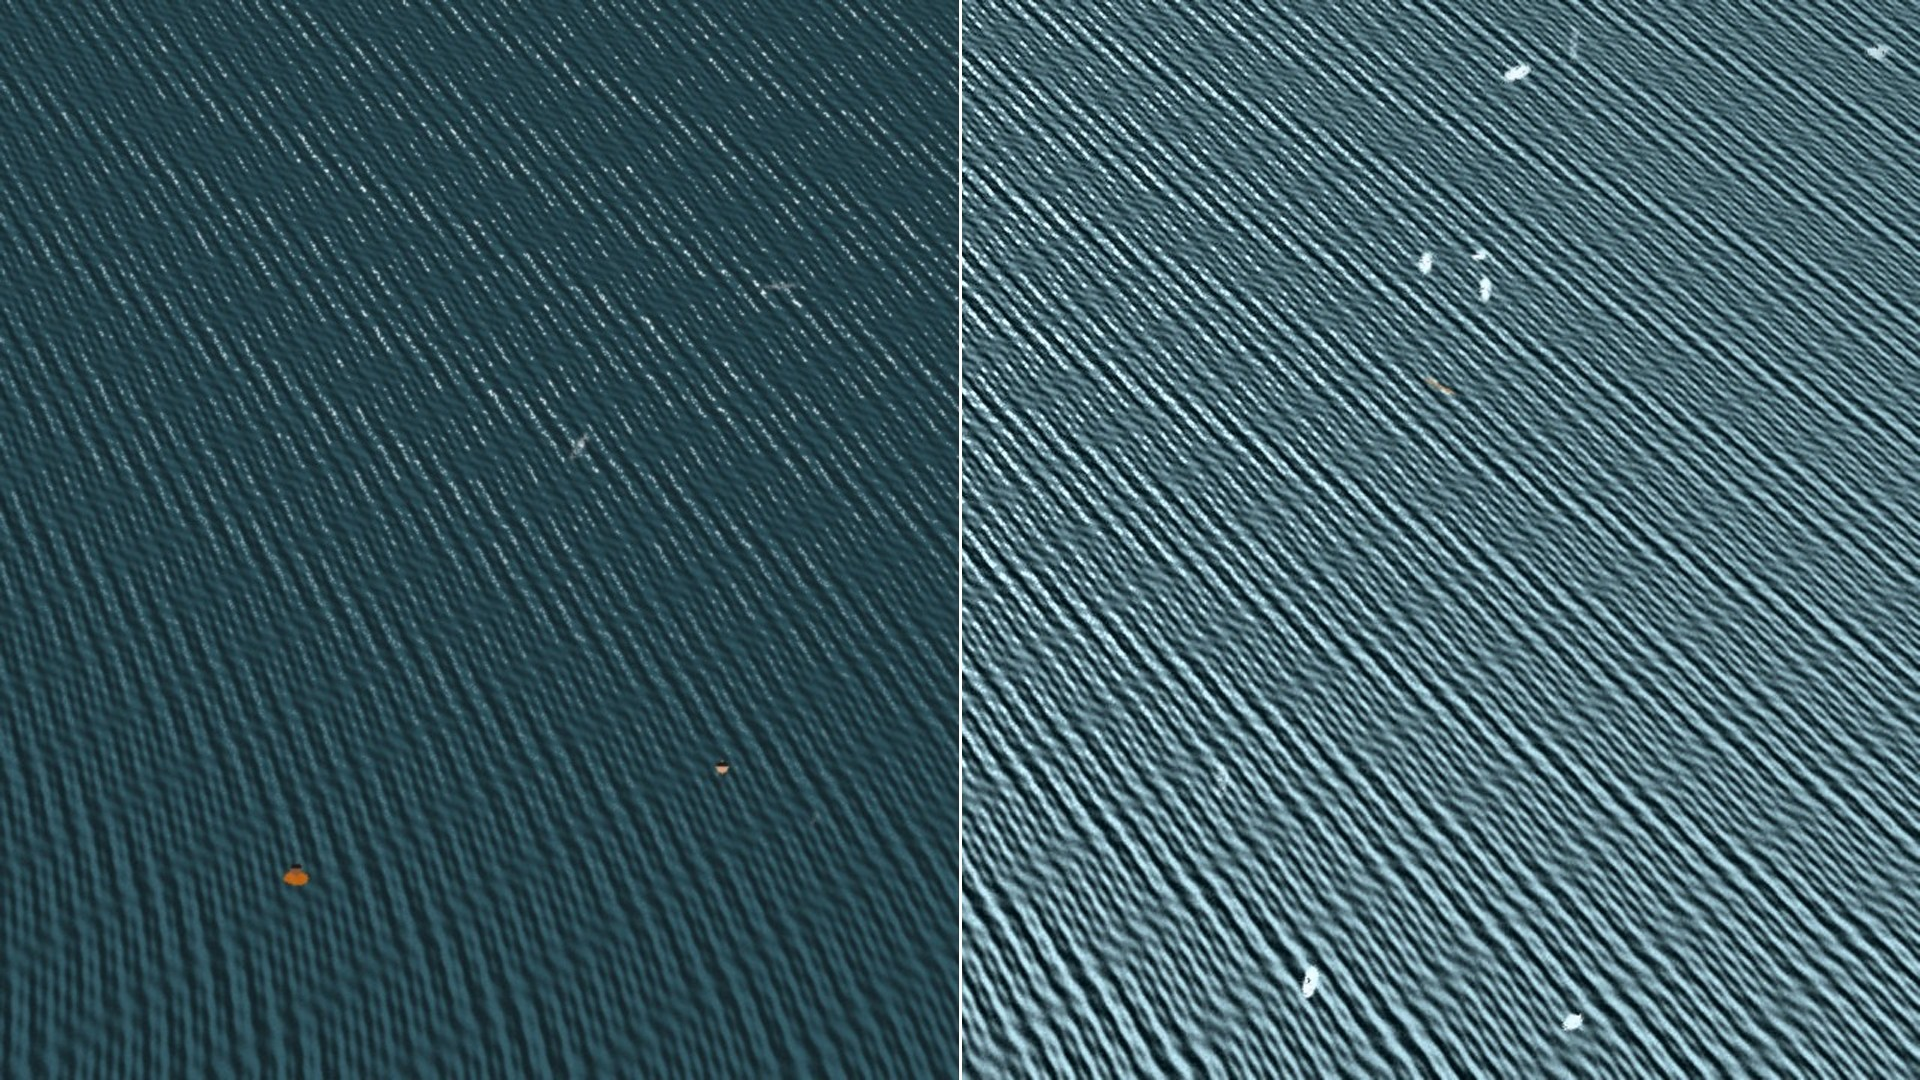
\includegraphics[width=0.72\textwidth]{norm_split.jpg}
\caption{The same frame before (left) and after (right) normalisation.}
\label{fig:norm}
\end{figure}

\subsection{Frequency-Domain Wave Estimate}

The frame is split into 3 horizontal bands, and the 2-D DFT of a Hann-windowed patch gives each band's power spectrum. The strongest peak with a wavelength of 4--32 px gives the dominant wavelength and orientation. This tunes the Gabor filters to the sea actually in the frame.

\subsection{Gabor Filtering}

For each distinct band wavelength, the bank has 4 orientations: the dominant one, then $+45^\circ$, $+90^\circ$ and $+135^\circ$, with $\sigma = 0.56\lambda$ and $\gamma = 0.5$. Each filter runs as an even and odd pair, and the local energy $\sqrt{\mathrm{even}^2 + \mathrm{odd}^2}$ does not depend on wave phase.

\begin{figure}[H]
\centering

\includegraphics[width=0.72\textwidth]{kernels.png}
\caption{Even Gabor kernels at the four orientations of one wavelength.}
\label{fig:kernels}
\end{figure}

\subsection{Uniform Local Binary Patterns}

Each pixel gets an 8-neighbour code (bit = neighbour $\geq$ centre), mapped to the 59 uniform bins~\cite{ojala}. A normalised LBP histogram per tile describes micro-texture without depending on absolute brightness. Tiles overlap by half, so a person on a tile border is not split.

\subsection{Median Filtering and Colour Distance}

The local sea colour is a median-filtered background. Pixels are measured against it in Lab space to turn an anomalous tile into a pixel-accurate candidate blob.

\subsection{Glint Suppression by Chromaticity}

Specular glint saturates all channels together, so its rgb chromaticity $(R, G, B) / (R + G + B)$ sits close to $(1/3, 1/3, 1/3)$. A pixel is glint if its mean is at least $0.8 \cdot 255$ and its distance from grey is at most 0.06. Requiring both keeps dark, colourless targets such as a black wetsuit.

\subsection{Morphological Filtering}

Opening ($3 \times 3$ ellipse) removes specks, and closing ($5 \times 5$) joins the fragments of a partly submerged body. Connected components (8-connectivity) must then pass three shape tests: area of 12--2,500 px, eccentricity $\leq$ 0.97 and solidity $\geq$ 0.45.

\begin{figure}[H]
\centering
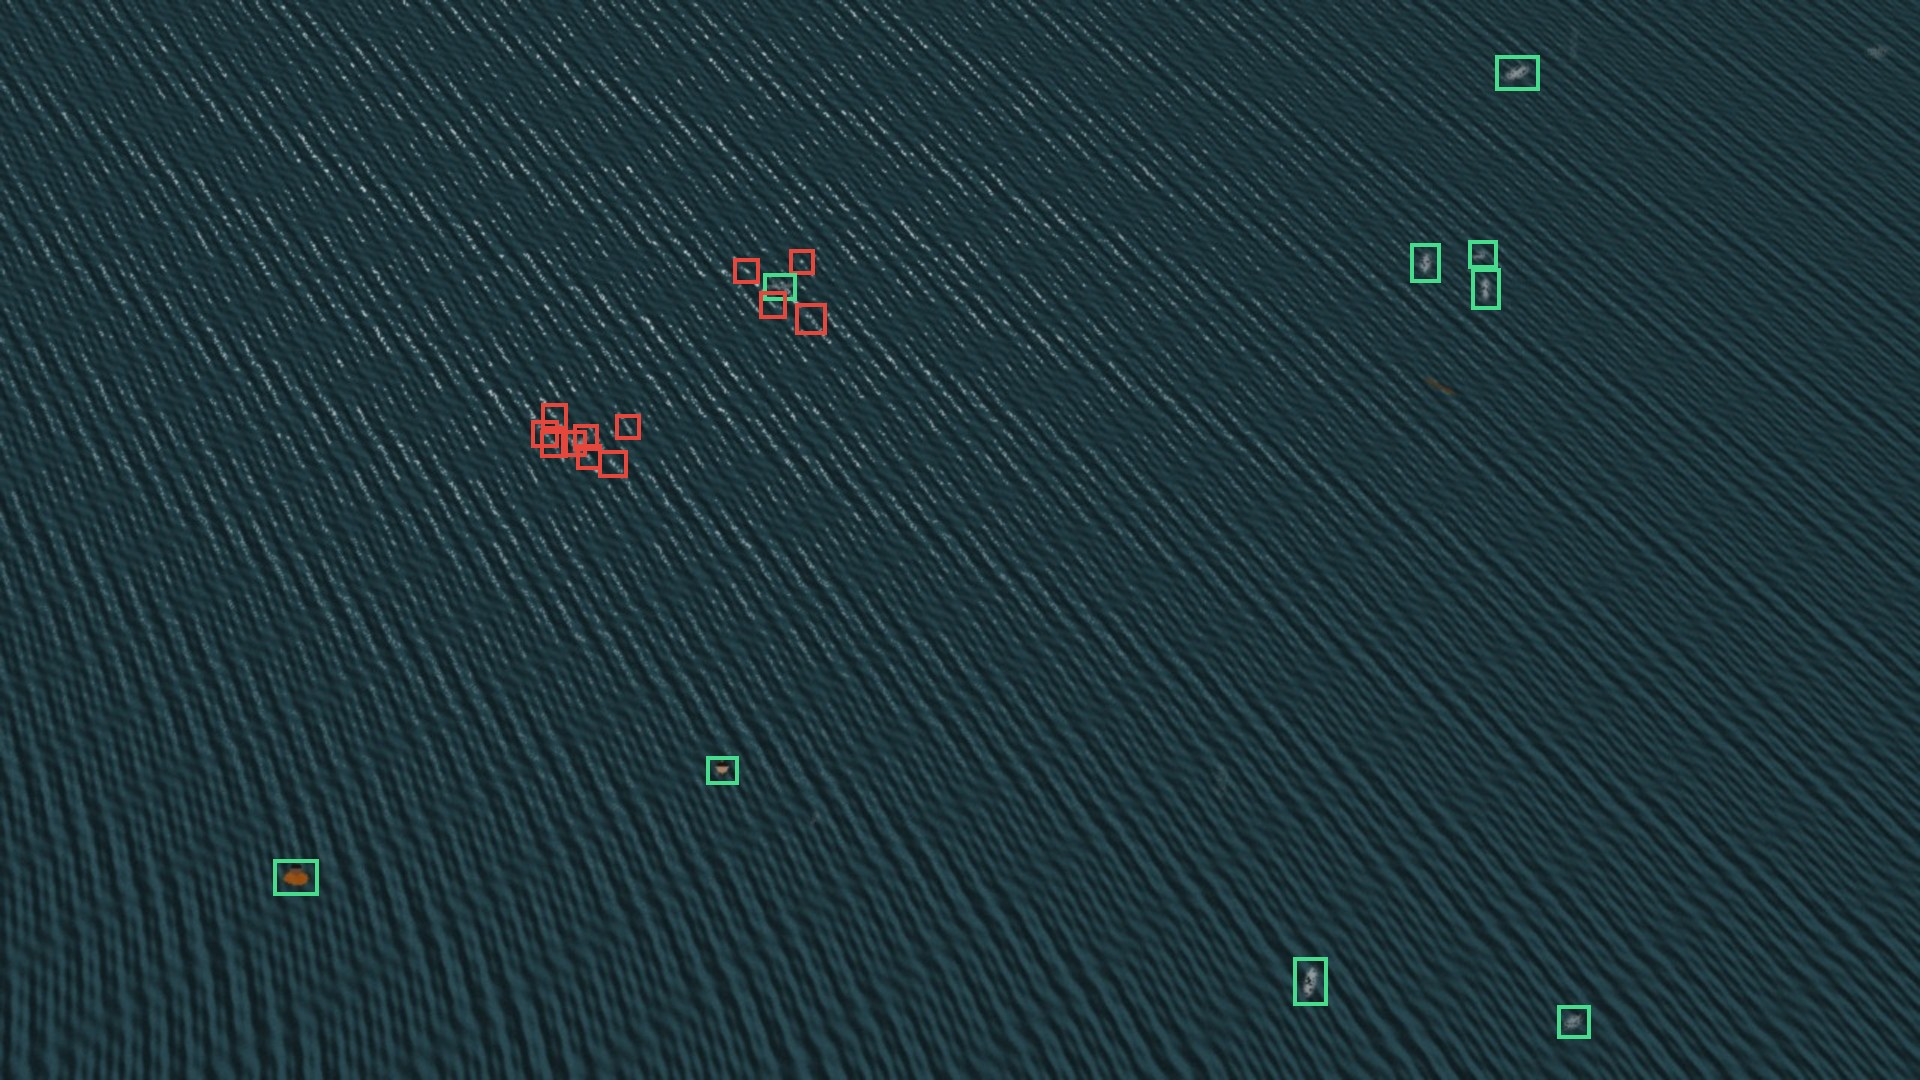
\includegraphics[width=0.72\textwidth]{morph_blobs.jpg}
\caption{Blobs after morphology: green passed the shape filter and red were rejected.}
\label{fig:morph}
\end{figure}

\subsection{Mapping to Lab Sessions 1--5}

\begin{table}[H]
\centering
\small
\caption{Lab techniques and where each is implemented.}
\label{tab:labs}
\begin{tabularx}{\textwidth}{@{}YY@{}}
\toprule
Technique & Implemented in \\
\midrule
Intensity transform: piecewise-linear contrast stretch & \texttt{normalise.piecewise\_linear} \\
Histogram processing: CLAHE & \texttt{normalise.normalise} \\
Spatial filtering: Gaussian, median, Gabor convolution & \texttt{normalise.flat\_field}, \texttt{anomaly.colour\_deviation}, \texttt{texture.gabor\_energy} \\
Frequency domain: 2-D DFT power spectrum & \texttt{texture.estimate\_wave} \\
Texture: uniform LBP, chi-square histogram distance & \texttt{texture.uniform\_lbp}, \texttt{anomaly.chi\_square} \\
Colour spaces: Lab, normalised rgb chromaticity & \texttt{anomaly.colour\_deviation}, \texttt{glint.chromaticity} \\
Thresholding: robust median + $k \cdot$MAD & \texttt{anomaly.score\_anomalies} \\
Morphology: opening, closing, structuring elements & \texttt{morphology.refine} \\
Connected components, moments, convex hull & \texttt{morphology.refine}, \texttt{eccentricity}, \texttt{solidity} \\
\bottomrule
\end{tabularx}
\end{table}

% ------------------------------------------------------------ code
\section{VS Code for Functional Design}

The functional design is a Python package, \texttt{sarvision}, with one module per stage and one shared configuration, so the GUI, command line and evaluation all run the same pipeline. The package is about 2,900 lines, and all 40 tests pass.

\subsection{Project Structure}

\begin{table}[H]
\centering
\small
\caption{Modules of the \texttt{sarvision} package.}
\label{tab:modules}
\begin{tabularx}{\textwidth}{@{}lY@{}}
\toprule
File & Responsibility \\
\midrule
\texttt{config.py} & Every tunable parameter, shared by GUI, CLI and evaluation \\
\texttt{normalise.py} & Stage 1: flat-fielding, CLAHE, contrast stretch \\
\texttt{texture.py} & Stage 2: wave spectrum, Gabor bank, uniform LBP, tile descriptors \\
\texttt{anomaly.py} & Stage 3: robust reference, chi-square distances, z-score fusion, candidate pixels \\
\texttt{glint.py} & Stage 4: chromaticity glint test \\
\texttt{morphology.py} & Stage 5: opening, closing, connected components, shape filter \\
\texttt{tracking.py} & Stage 6: association, persistence, drift test, ranking \\
\texttt{pipeline.py} & Runs the stages in order; optional camera-motion compensation \\
\texttt{gui.py}, \texttt{viz.py} & Tkinter operator GUI; stage rendering and overlay \\
\texttt{datasets.py}, \texttt{metrics.py}, \texttt{evaluate.py} & Dataset loaders, metrics, ablations, plots \\
\texttt{synthetic.py} & Synthetic sea sequences with ground truth \\
\texttt{tests/} & Unit tests for each stage and end-to-end tests \\
\bottomrule
\end{tabularx}
\end{table}

\subsection{Running the Application}

\begin{lstlisting}[language=bash]
pip install -r requirements.txt
python -m sarvision synth --out data/synthetic
python -m sarvision gui data/synthetic/seq02.mp4
python -m sarvision run --input data/synthetic/seq02.mp4 --output results/demo/seq02_annotated.mp4 --csv results/demo/seq02_shortlist.csv
python -m sarvision evaluate --coco data/synthetic/annotations.json --ablations full,no_temporal,no_glint,no_morphology --out results/synthetic
python -m pytest -q
\end{lstlisting}

\subsection{Key Code}

\needspace{15\baselineskip}
\textbf{Stage 1: normalisation} (\texttt{normalise.py})

\begin{lstlisting}[language=Python]
def normalise(bgr: np.ndarray, cfg: Config) -> tuple[np.ndarray, np.ndarray]:
    """Return (normalised BGR frame, normalised grey frame), both uint8."""
    lab = cv2.cvtColor(bgr, cv2.COLOR_BGR2LAB)
    l_chan, a_chan, b_chan = cv2.split(lab)
    l_flat = flat_field(l_chan, cfg.flatten_sigma)
    clahe = cv2.createCLAHE(clipLimit=cfg.clahe_clip, tileGridSize=(cfg.clahe_grid, cfg.clahe_grid))
    l_eq = clahe.apply(l_flat)
    l_st = contrast_stretch(l_eq, cfg)
    bgr_n = cv2.cvtColor(cv2.merge([l_st, a_chan, b_chan]), cv2.COLOR_LAB2BGR)
    return bgr_n, l_st
\end{lstlisting}

\needspace{24\baselineskip}
\textbf{Stage 2: Gabor energy and LBP codes} (\texttt{texture.py})

\begin{lstlisting}[language=Python]
def gabor_energy(gray: np.ndarray, filt: GaborFilter) -> np.ndarray:
    """Local energy sqrt(even^2 + odd^2): phase-invariant response magnitude."""
    f = gray.astype(np.float32)
    e = cv2.filter2D(f, cv2.CV_32F, filt.even, borderType=cv2.BORDER_REFLECT)
    o = cv2.filter2D(f, cv2.CV_32F, filt.odd, borderType=cv2.BORDER_REFLECT)
    return cv2.magnitude(e, o)

def lbp_codes(gray: np.ndarray) -> np.ndarray:
    """Basic 8-neighbour LBP: bit i is 1 if neighbour i >= centre."""
    g = gray.astype(np.int16)
    p = np.pad(g, 1, mode="edge")
    h, w = g.shape
    code = np.zeros((h, w), dtype=np.uint8)
    for bit, (dy, dx) in enumerate(_NEIGHBOURS):
        nb = p[1 + dy:1 + dy + h, 1 + dx:1 + dx + w]
        code |= ((nb >= g).astype(np.uint8) << bit)
    return code
\end{lstlisting}

\needspace{15\baselineskip}
\textbf{Stage 3: distance and robust score} (\texttt{anomaly.py})

\begin{lstlisting}[language=Python]
def chi_square(a: np.ndarray, b: np.ndarray) -> np.ndarray:
    """0.5 * sum((a - b)^2 / (a + b)) over the last axis."""
    return 0.5 * np.sum((a - b) ** 2 / (a + b + EPS), axis=-1)

def robust_z(x: np.ndarray) -> np.ndarray:
    med = np.median(x)
    mad = np.median(np.abs(x - med)) * MAD_TO_SIGMA
    if mad < EPS:
        mad = x.std() + EPS
    return (x - med) / mad
\end{lstlisting}

\needspace{14\baselineskip}
\textbf{Stage 4: glint mask} (\texttt{glint.py})

\begin{lstlisting}[language=Python]
def glint_mask(bgr: np.ndarray, cfg: Config) -> np.ndarray:
    """Boolean mask of bright, achromatic pixels."""
    total = bgr.astype(np.uint16).sum(axis=-1)
    bright = total >= 3.0 * 255.0 * cfg.glint_value
    out = np.zeros(bright.shape, dtype=bool)
    if bright.any():
        px = bgr[bright]
        out[bright] = chroma_distance(px[None])[0] <= cfg.glint_chroma
    return out
\end{lstlisting}

\needspace{13\baselineskip}
\textbf{Stage 5: opening and closing} (\texttt{morphology.py}, excerpt from \texttt{refine})

\begin{lstlisting}[language=Python]
if cfg.open_ksize > 1:
    k = cv2.getStructuringElement(cv2.MORPH_ELLIPSE, (cfg.open_ksize, cfg.open_ksize))
    work = cv2.morphologyEx(work, cv2.MORPH_OPEN, k)
if cfg.close_ksize > 1:
    k = cv2.getStructuringElement(cv2.MORPH_ELLIPSE, (cfg.close_ksize, cfg.close_ksize))
    work = cv2.morphologyEx(work, cv2.MORPH_CLOSE, k)

n, labels, stats, cents = cv2.connectedComponentsWithStats(work, connectivity=8)
\end{lstlisting}

\needspace{21\baselineskip}
\textbf{Stage 6: ranking} (\texttt{tracking.py})

\begin{lstlisting}[language=Python]
def ranked(self, frame: int) -> list[RankedCandidate]:
    """Promoted tracks ranked by the combined anomaly/persistence confidence."""
    cfg = self.cfg
    out = []
    for t in self.tracks:
        coh = t.coherence(cfg)
        if t.hits < cfg.min_persistence or coh < cfg.min_coherence:
            continue
        missed = frame - t.last_frame
        persist = min(t.hits, cfg.persistence_horizon) / float(cfg.persistence_horizon) * coh
        conf = cfg.anomaly_weight * t.conf_ema + (1.0 - cfg.anomaly_weight) * persist
        conf *= 0.8 ** missed
        out.append(RankedCandidate(t.det, float(conf), t.tid, t.hits, coh, missed))
    out.sort(key=lambda c: -c.conf)
    return out
\end{lstlisting}

% ------------------------------------------------------------ references
\addcontentsline{toc}{section}{References}
\begin{thebibliography}{10}

\bibitem{gonzalez} R. C. Gonzalez and R. E. Woods, \emph{Digital Image Processing}, 3rd ed. Pearson Education, 2012.

\bibitem{szeliski} R. Szeliski, \emph{Computer Vision: Algorithms and Applications}. Springer, 2011.

\bibitem{sonka} M. Sonka, V. Hlavac and R. Boyle, \emph{Digital Image Processing and Computer Vision}, India ed. Cengage Learning, 2009.

\bibitem{howse} J. Howse, P. Joshi and M. Beyeler, \emph{OpenCV: Computer Vision Projects with Python}. Packt Publishing, 2016.

\bibitem{baggio} D. L. Baggio, S. Emami, D. M. Escriv\'a, K. Ievgen, N. Mahmood, J. Saragih and R. Shilkrot, \emph{Mastering OpenCV 3}, 2nd ed. Packt Publishing, 2017.

\bibitem{laganiere} R. Laganiere, \emph{OpenCV Computer Vision Application Programming Cookbook}, 2nd ed. Packt Publishing, 2014.

\bibitem{ojala} T. Ojala, M. Pietik\"ainen and T. M\"aenp\"a\"a, ``Multiresolution gray-scale and rotation invariant texture classification with local binary patterns,'' \emph{IEEE Transactions on Pattern Analysis and Machine Intelligence}, vol. 24, no. 7, pp. 971--987, 2002. \href{https://doi.org/10.1109/TPAMI.2002.1017623}{doi:10.1109/TPAMI.2002.1017623}

\bibitem{seadronessee} L. A. Varga, B. Kiefer, M. Messmer and A. Zell, ``SeaDronesSee: A Maritime Benchmark for Detecting Humans in Open Water,'' in \emph{Proc. IEEE/CVF Winter Conference on Applications of Computer Vision (WACV)}, 2022, pp. 2260--2270.

\bibitem{mobdrone} D. Cafarelli et al., ``MOBDrone: A Drone Video Dataset for Man OverBoard Rescue,'' in \emph{Image Analysis and Processing -- ICIAP 2022}. Springer, 2022, pp. 633--644.

\bibitem{afo} J. G\k{a}sienica-J\'ozkowy, M. Knapik and B. Cyganek, ``An ensemble deep learning method with optimized weights for drone-based water rescue and surveillance,'' \emph{Integrated Computer-Aided Engineering}, vol. 28, no. 3, pp. 221--235, 2021. \href{https://doi.org/10.3233/ICA-210649}{doi:10.3233/ICA-210649}

\end{thebibliography}

\end{document}
